
\documentclass[10pt,twoside]{article}   	% use "amsart" instead of "article" for AMSLaTeX format
\usepackage{geometry}                		% See geometry.pdf to learn the layout options. There are lots.
\geometry{a4paper, bottom=2.5cm, top=2cm, left=2cm, right=2cm}                   		% ... or a4paper or a5paper or ... 
%\geometry{landscape}                		% Activate for rotated page geometry
%\usepackage[parfill]{parskip}    		% Activate to begin paragraphs with an empty line rather than an indent
\usepackage{graphicx,subfigure, array}				% Use pdf, png, jpg, or eps§ with pdflatex; use eps in DVI mode
								% TeX will automatically convert eps --> pdf in pdflatex	
\usepackage{amssymb}
\usepackage{amsmath}
\usepackage{verbatim}
\usepackage{tikz}
\usetikzlibrary{arrows,shapes}
\usepackage{listings}
\usepackage{color}
\usepackage{hyperref,url}
\usepackage[hang,  bf, margin=19pt, tableposition=top,textfont=it]{caption}
\usepackage{algorithm}
\usepackage{algpseudocode}
\usepackage{multicol,multirow}
\usepackage{subfigure}
\usepackage{fancyvrb,newverbs,xcolor}


% COMMANDS
\newcommand{\N}{\mathbb{N}} 
\newtheorem{theorem}{Theorem}
\newtheorem{definition}{Definition}
\newtheorem{lemma}{Lemma}
\newtheorem{corollary}{Corollary}
\newtheorem{property}{Property}
\newtheorem{proof}{Proof}

\newlength{\textlarg}
\newcommand{\barre}[1]{%
   \settowidth{\textlarg}{#1}
   #1\hspace{-\textlarg}\rule[0.5ex]{\textlarg}{0.5pt}}


\algnewcommand\algorithmicswitch{\textbf{switch}}
\algnewcommand\algorithmiccase{\textbf{case}}
\algnewcommand\algorithmicassert{\texttt{break}}
\algnewcommand\Break[1]{\State \algorithmicbreak(#1)}%
% New "environments"
\algdef{SE}[SWITCH]{Switch}{EndSwitch}[1]{\algorithmicswitch\ #1\ \algorithmicdo}{\algorithmicend\ \algorithmicswitch}%
\algdef{SE}[CASE]{Case}{EndCase}[1]{\algorithmiccase\ #1}{\algorithmicend\ \algorithmiccase}%
\algtext*{EndSwitch}%
\algtext*{EndCase}%


% COLORS
\definecolor{bleugris}{RGB}{43,78,103}
\definecolor{codegreen}{rgb}{0.56,0.74,0.56}
\definecolor{backcolor}{rgb}{0.95,0.95,0.96}
\definecolor{lightgray}{gray}{0.35}
\definecolor{codegray}{rgb}{0.5,0.5,0.5}
\definecolor{codered}{rgb}{0.87,0.19,0.39}
\definecolor{cverbbg}{gray}{0.93}

\newenvironment{cverbatim}
 {\SaveVerbatim{cverb}}
 {\endSaveVerbatim
  \flushleft\fboxrule=0pt\fboxsep=.5em
  \colorbox{cverbbg}{\BUseVerbatim{cverb}}%
  \endflushleft
}
\newenvironment{lcverbatim}
 {\SaveVerbatim{cverb}}
 {\endSaveVerbatim
  \flushleft\fboxrule=0pt\fboxsep=.5em
  \colorbox{cverbbg}{%
    \makebox[\dimexpr\linewidth-2\fboxsep][l]{\BUseVerbatim{cverb}}%
  }
  \endflushleft
}

\newcommand{\ctexttt}[1]{\colorbox{cverbbg}{\texttt{#1}}}
\newverbcommand{\cverb}
  {\setbox\verbbox\hbox\bgroup}
  {\egroup\colorbox{cverbbg}{\box\verbbox}}




\lstdefinestyle{mystyle}{
	%backgroundcolor=\color{backcolor},
	commentstyle=\color{codegreen},
	keywordstyle=\color{codered},
	numberstyle=\tiny\color{codegray},
	basicstyle=\scriptsize,
	breaklines=true,
	breakatwhitespace=false,
	numbers=left,
	tabsize=2
}

\lstset{style=mystyle}


\DeclareCaptionFont{white}{\color{white}}
\DeclareCaptionFormat{listing}{\colorbox[cmyk]{0.43, 0.35, 0.35,0.01}{\parbox{\textwidth}{\hspace{15pt}#3}}}
\DeclareCaptionFormat{listing2}{\colorbox[cmyk]{0.9, 0.9, 0.9,0.01}{\parbox{\textwidth}{\hspace{15pt}#3}}}
\captionsetup[lstlisting]{format=listing,labelfont=white,textfont=white,singlelinecheck=false,margin=0pt,font={bf}}


\title{Hou10ni Profiling with TAU}
\date{}						



\begin{document}
\maketitle

This document presents some results obtained with the performance evaluation tool TAU on the application hou10ni.

\section{How to use TAU on hou10ni}

\begin{cverbatim}
export TAU_MAKEFILE=$TAU_DIR/Makefile.
export TAU_OPTIONS='-optPdtF95Opts="-R free" -optVerbose'

cd build
cmake ..
ccmake ..
\end{cverbatim}

\noindent $\rightarrow$ Press "t" to change the compiler and chose \texttt{tau\_f90.sh}. Then you can tape \texttt{make} and launch the application.

\begin{cverbatim}
make
cd .. 
mpirun -np 4 tau_exec -T mpi  build/hou10ni.out < HPC4E.dat
\end{cverbatim}

\noindent To visualize the results with paraprof, 
\begin{cverbatim}
paraprof &
\end{cverbatim}
or
\begin{cverbatim}
paraprof --pack app.ppk
\end{cverbatim}
This last command will create the file \texttt{app.ppk}.

\section{Trace Visualisation with Jumpshot tool}

Jumpshot user guide: \url{ftp://ftp.mcs.anl.gov/pub/mpi/slog2/js4-usersguide.pdf}\\

\noindent To generate a trace of an application, follow the steps presented below.

\begin{cverbatim}
export TAU_TRACE=1
mpirun -np 4 tau_exec -T mpi  build/hou10ni.out < HPC4E.dat
tau_treemerge.pl
\end{cverbatim}

\noindent $\rightarrow$ Two files are created:  tau.trc and tau.edf

\begin{cverbatim}
tau2slog2 tau.trc tau.edf  -o app.slog2
jumpshot app.slog2
\end{cverbatim}

Figure \ref{fig:trace} shows the trace obtained with 4 MPI processes, TAU instrumentation and displayed with the Jumpshot tool. Figure \ref{fig:trace2} presents a zoom on the big portion and Figure \ref{fig:trace3} depicts the end of the trace. The purple/pink color represents the \texttt{MPI\_Wait} function. In Figure \ref{fig:trace3} we can see the different time spent in \texttt{MPI\_Wait} for all processes.

\begin{figure}[ht!]
\centering
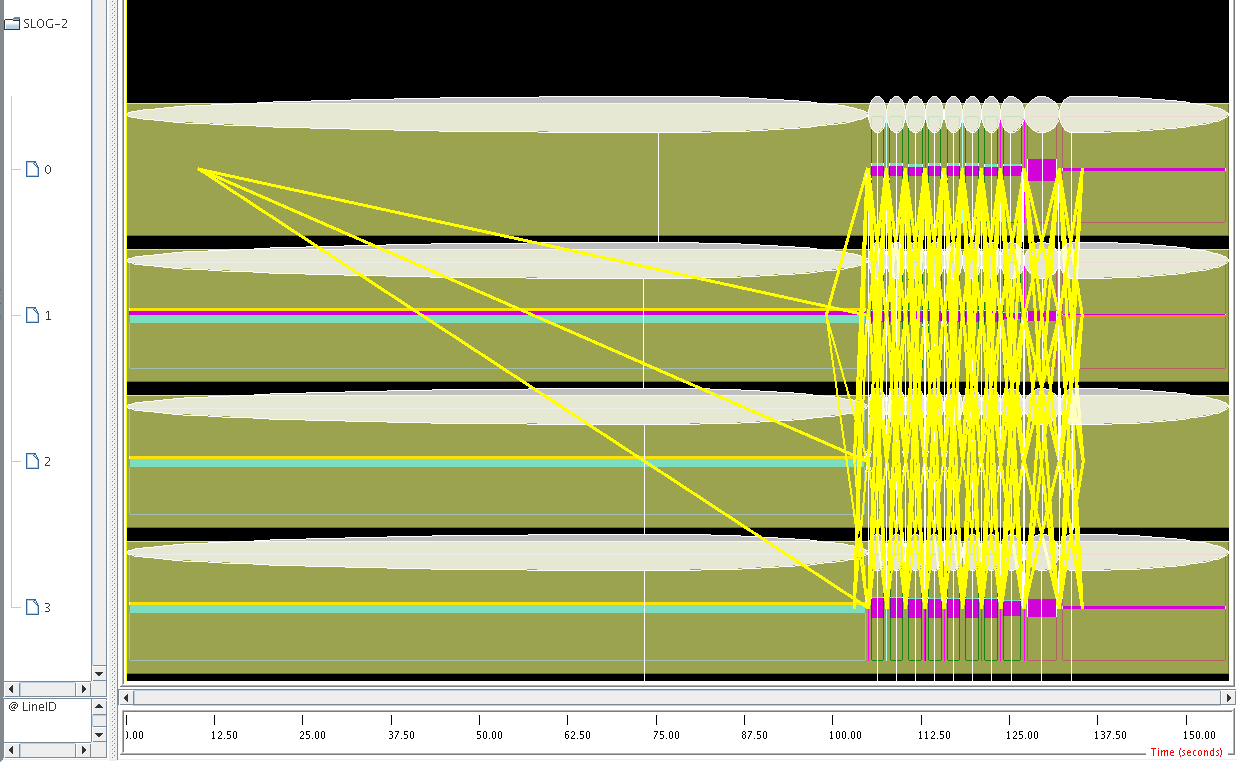
\includegraphics[width=13cm]{IMAGES/jumpshot1}
\caption{Trace Visualisation with Jumpshot}
\label{fig:trace}
\end{figure}

\begin{figure}[ht!]
\centering
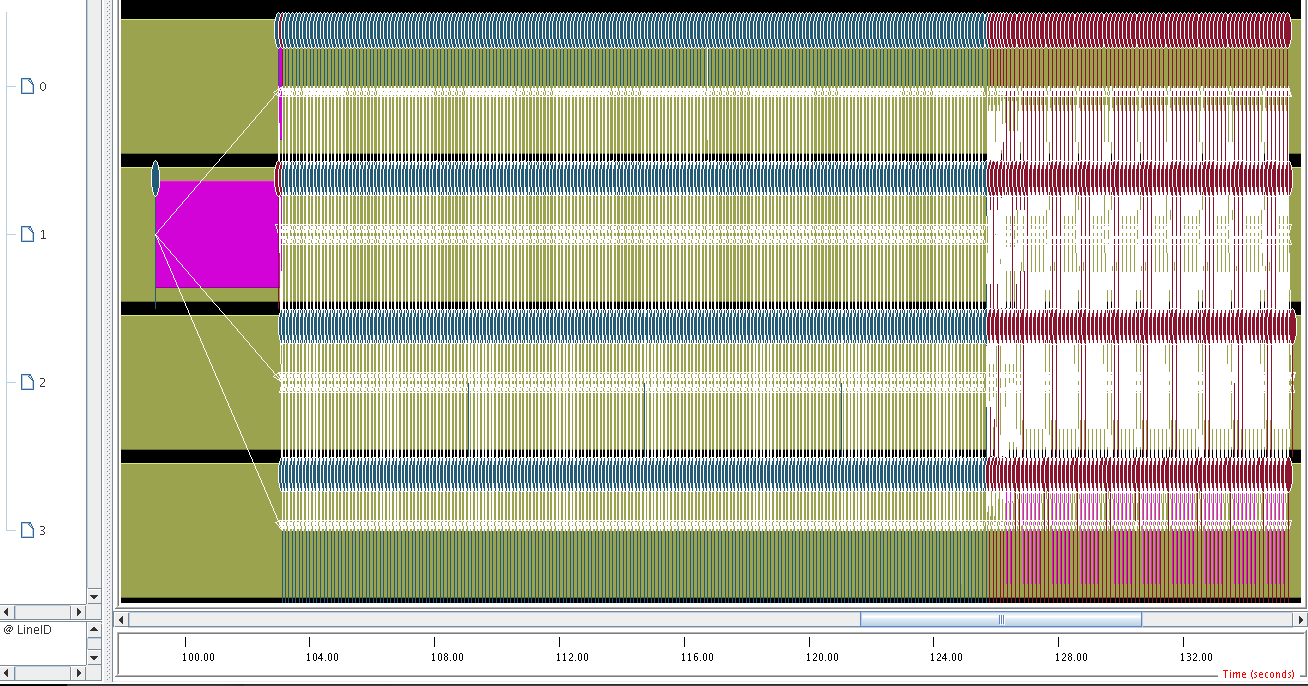
\includegraphics[width=13cm]{IMAGES/jumpshot2}
\caption{Zoom on the big portion in Figure \ref{fig:trace}}
\label{fig:trace2}
\end{figure}

\begin{figure}[ht!]
\centering
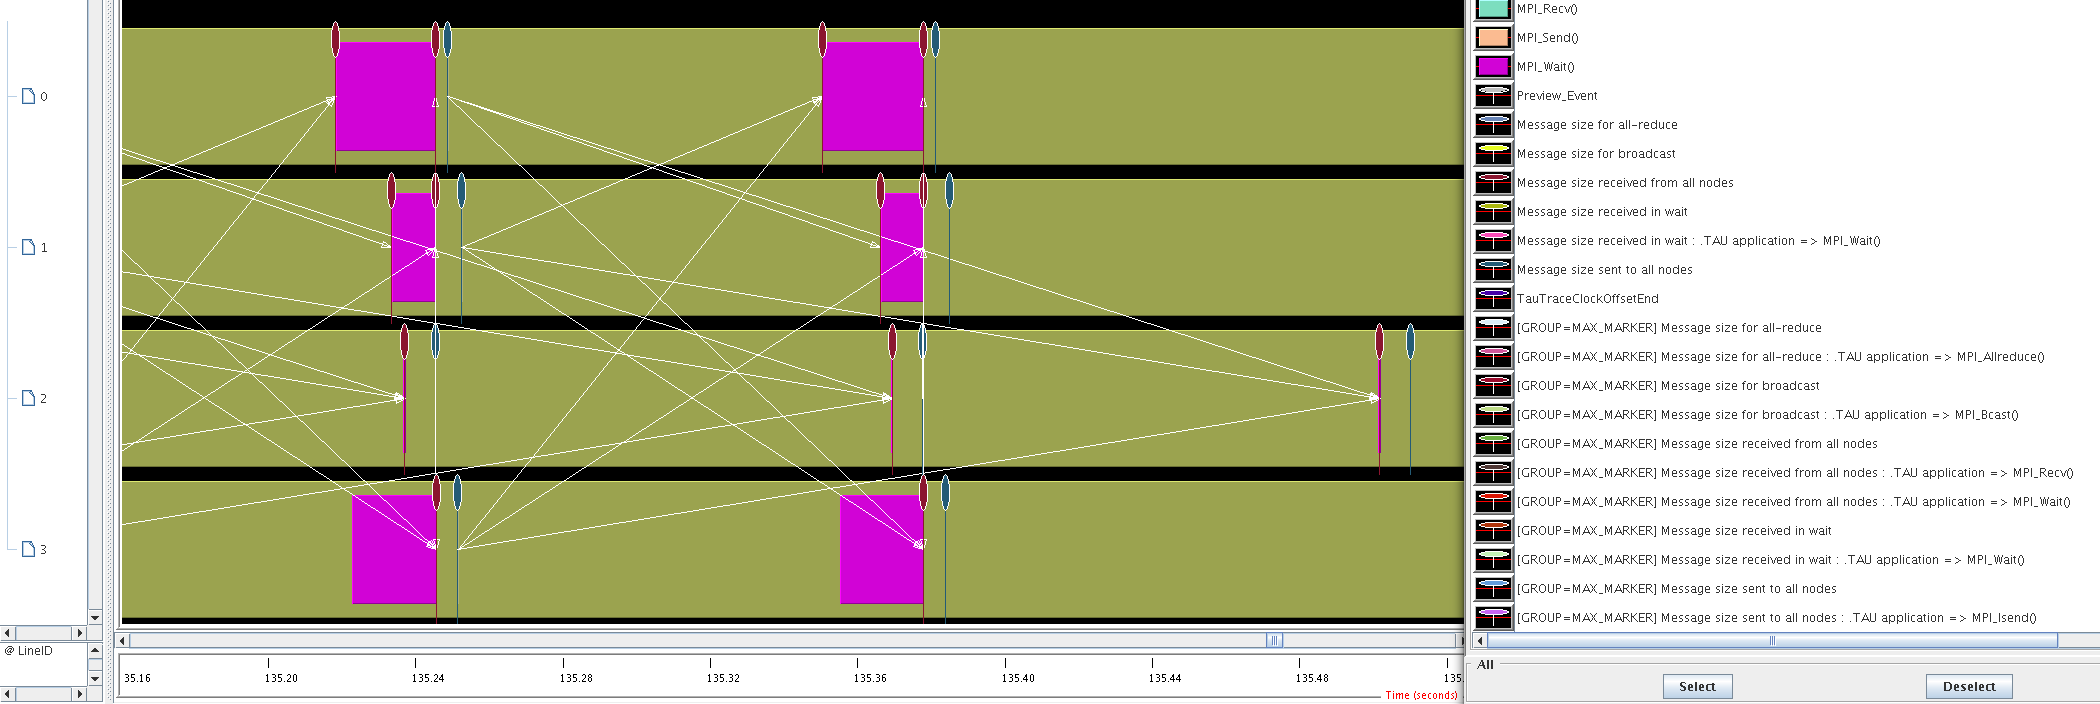
\includegraphics[width=15cm]{IMAGES/jumpshot3}
\caption{Zoom on the end of the trace}
\label{fig:trace3}
\end{figure}

%\begin{figure}[ht!]
%\centering
%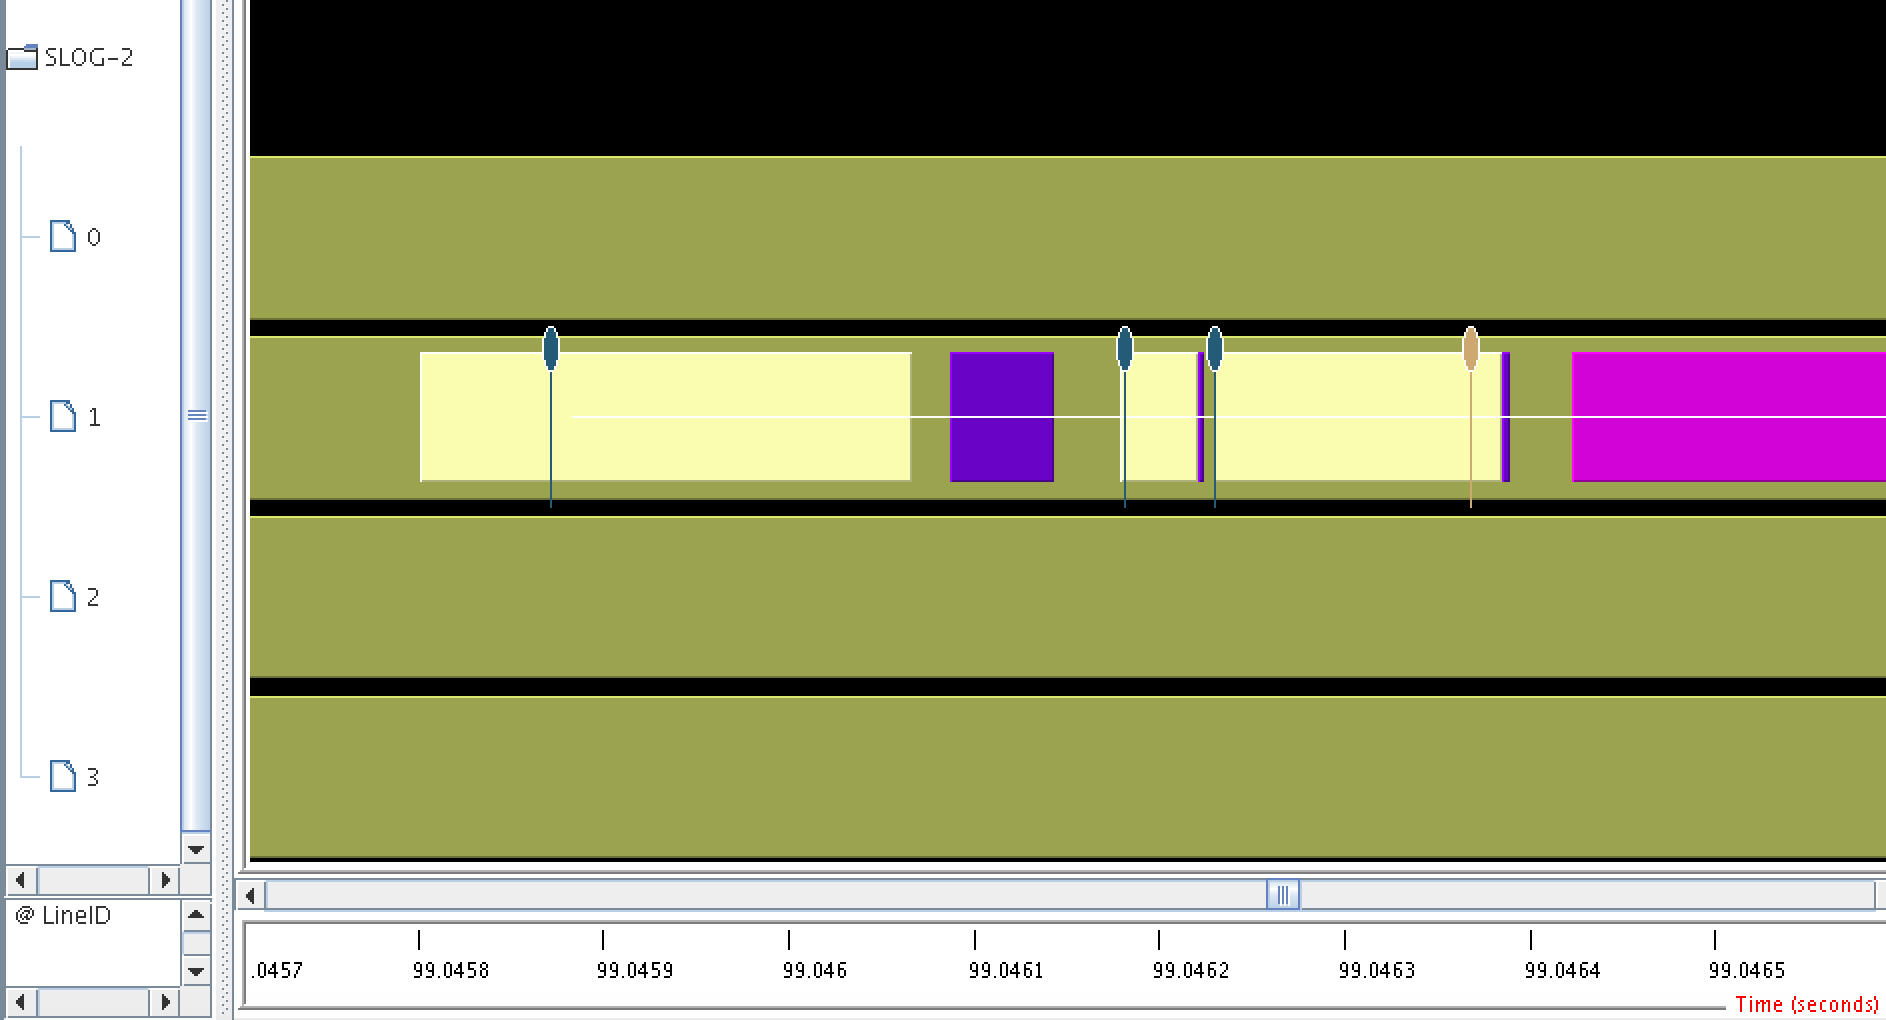
\includegraphics[width=10cm]{IMAGES/jumpshot4}
%\caption{Zoom on the beginning of the trace}
%\label{fig:trace3}
%\end{figure}

\section{Profile Visualisation with paraprof}


It is possible to get a detailed summary in a text format. To record all information in a file \textit{profile\_summary.txt}, the command is
\begin{cverbatim}
pprof > profile_summary.txt
\end{cverbatim}

\noindent The file created looks like the following

{\scriptsize
\begin{verbatim}
Reading Profile files in profile.*

NODE 0;CONTEXT 0;THREAD 0:
---------------------------------------------------------------------------------------
%Time    Exclusive    Inclusive       #Call      #Subrs  Inclusive Name
              msec   total msec                          usec/call
---------------------------------------------------------------------------------------
 72.9            0     2:02.995       12300           0      10000 .TAU application => [CONTEXT] .TAU application
 72.9            0     2:02.995       12300           0      10000 [CONTEXT] .TAU application
 54.0     1:31.155     1:31.155        9116           0      10000 [SAMPLE] UNRESOLVED /lib64/libpthread-2.11.3.so
 54.0     1:31.122     1:31.122        9113           0       9999 .TAU application => [CONTEXT] .TAU application => [SAMPLE] UNRESOLVED ..
 23.3       39,314       39,314        1644           0      23914 MPI_Wait()
 23.3            0       39,300        3929           0      10003 MPI_Wait() => [CONTEXT] MPI_Wait()
 23.3            0       39,300        3929           0      10003 [CONTEXT] MPI_Wait()
 14.5       24,542       24,542        2454           0      10001 .TAU application => [CONTEXT] .TAU application => [SAMPLE] UNRESOLVED ..
 14.5       24,542       24,542        2454           0      10001 [SAMPLE] UNRESOLVED /home/esaillard/hou10ni2d/build/hou10ni.out
 10.7       18,132       18,132        1813           0      10002 [SAMPLE] MPID_nem_mpich_blocking_recv
 10.3       17,368       17,368        1737           0       9999 MPI_Wait() => [CONTEXT] MPI_Wait() => [SAMPLE] MPID_nem_mpich_blocking_recv
....


USER EVENTS Profile :NODE 0, CONTEXT 0, THREAD 0
---------------------------------------------------------------------------------------
NumSamples   MaxValue   MinValue  MeanValue  Std. Dev.  Event Name
---------------------------------------------------------------------------------------
         4          8          4          6          2  Message size for all-reduce
        76  1.375E+07          4  6.716E+05  2.489E+06  Message size for broadcast
      2022  5.426E+04          4  1.111E+04  1.929E+04  Message size received from all nodes
       822  5.426E+04       1024  2.732E+04  2.174E+04  Message size received in wait

....

NODE 1;CONTEXT 0;THREAD 0:
---------------------------------------------------------------------------------------
%Time    Exclusive    Inclusive       #Call      #Subrs  Inclusive Name
              msec   total msec                          usec/call
---------------------------------------------------------------------------------------
 93.7            0     2:38.072       15805           0      10001 .TAU application => [CONTEXT] .TAU application
 93.7            0     2:38.072       15805           0      10001 [CONTEXT] .TAU application
 61.9     1:44.423     1:44.423       10444           0       9998 [SAMPLE] UNRESOLVED /lib64/libpthread-2.11.3.so
 61.9     1:44.405     1:44.405       10443           0       9998 .TAU application => [CONTEXT] .TAU application => [SAMPLE] UNRESOLVED ..
 31.7       53,555       53,555        5351           0      10008 .TAU application => [CONTEXT] .TAU application => [SAMPLE] UNRESOLVED ..
 31.7       53,555       53,555        5351           0      10008 [SAMPLE] UNRESOLVED /home/esaillard/hou10ni2d/build/hou10ni.out
  4.2        7,074        7,074         424           0      16685 MPI_Recv()
  4.2            0        7,071         707           0      10002 MPI_Recv() => [CONTEXT] MPI_Recv()
  4.2            0        7,071         707           0      10002 [CONTEXT] MPI_Recv()
  3.0        5,135        5,135         516           0       9953 [SAMPLE] MPID_nem_mpich_blocking_recv
  2.3        3,807        3,807         380           0      10021 MPI_Recv() => [CONTEXT] MPI_Recv() => [SAMPLE] MPID_nem_mpich_blocking_recv
  1.5            0        2,550         255           0      10004 MPI_Bcast() => [CONTEXT] MPI_Bcast()
  1.5            0        2,550         255           0      10004 [CONTEXT] MPI_Bcast()
  1.5        2,543        2,543          76           0      33468 MPI_Bcast()

....
and so on
\end{verbatim}
}

\noindent Figures \ref{fig:1} and \ref{fig:2} show the entire application time with paraprof. 

\begin{figure}[H]
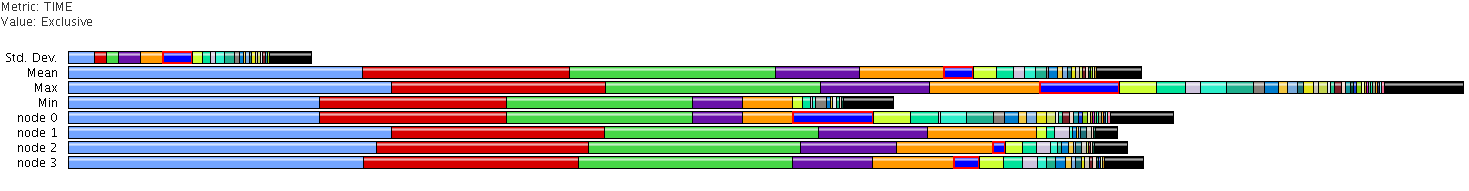
\includegraphics[width=18cm]{IMAGES/ScreenShot2}
\caption{Paraprof main window with stack bars together}
\label{fig:1}
\end{figure}

\begin{figure}[H]
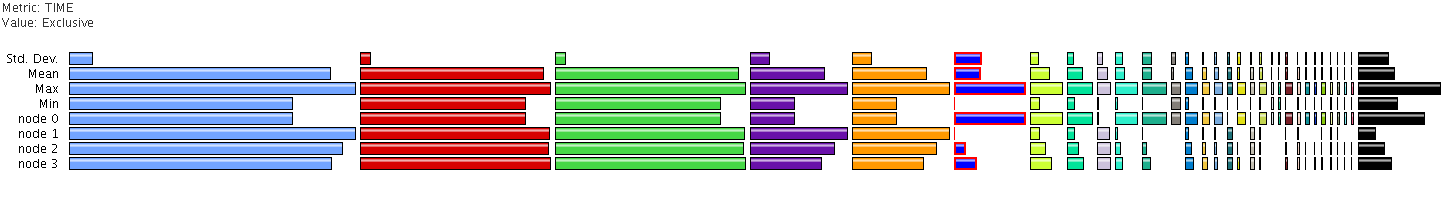
\includegraphics[width=18cm]{IMAGES/ScreenShot2bis}
\caption{Paraprof main window }
\label{fig:2}
\end{figure}

\begin{figure}[H]
\centering
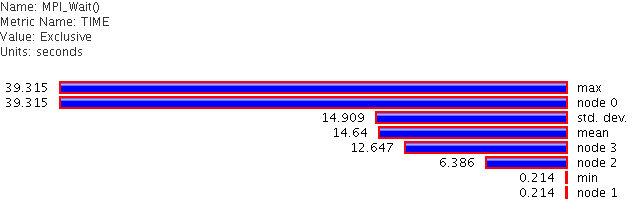
\includegraphics[width=10cm]{IMAGES/ScreenShotWait}
\caption{Time in one of MPI\_Wait function}
\label{fig:wait}
\end{figure}

\noindent {\bf{Statistics per process}} \\

\begin{figure}[H]
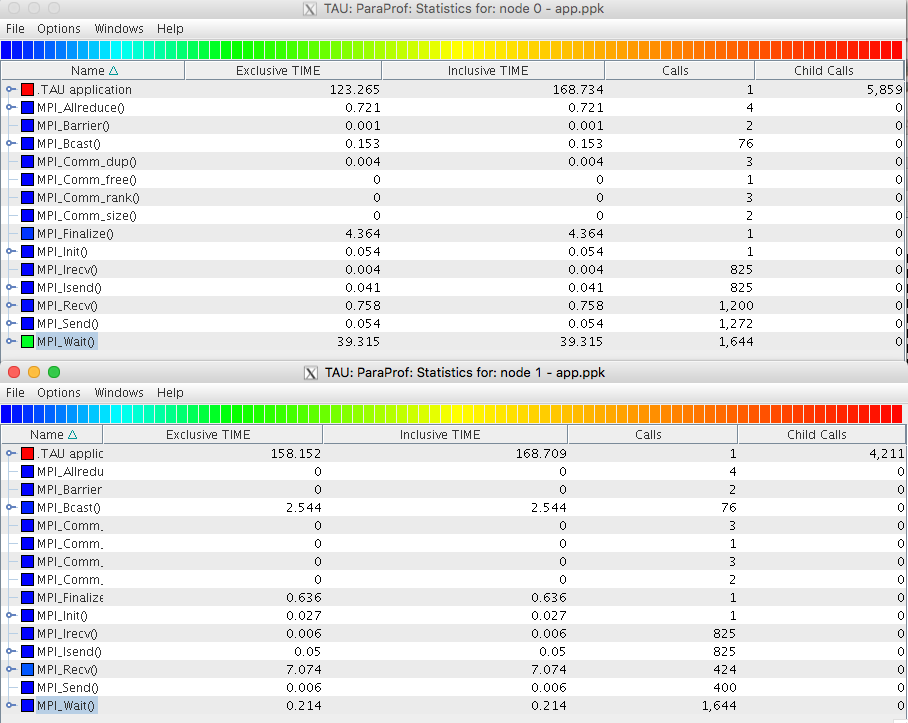
\includegraphics[width=18cm]{IMAGES/ScreenShot5}
\caption{Statistics for processes 0 and 1}
\label{fig:5}
\end{figure}

\noindent {\bf{Comparison Window}} \\

To get a comparison window, click right on the text \textit{node 0} for example and chose \textit{"Add Thread to Comparison Window"}.

\begin{figure}[H]
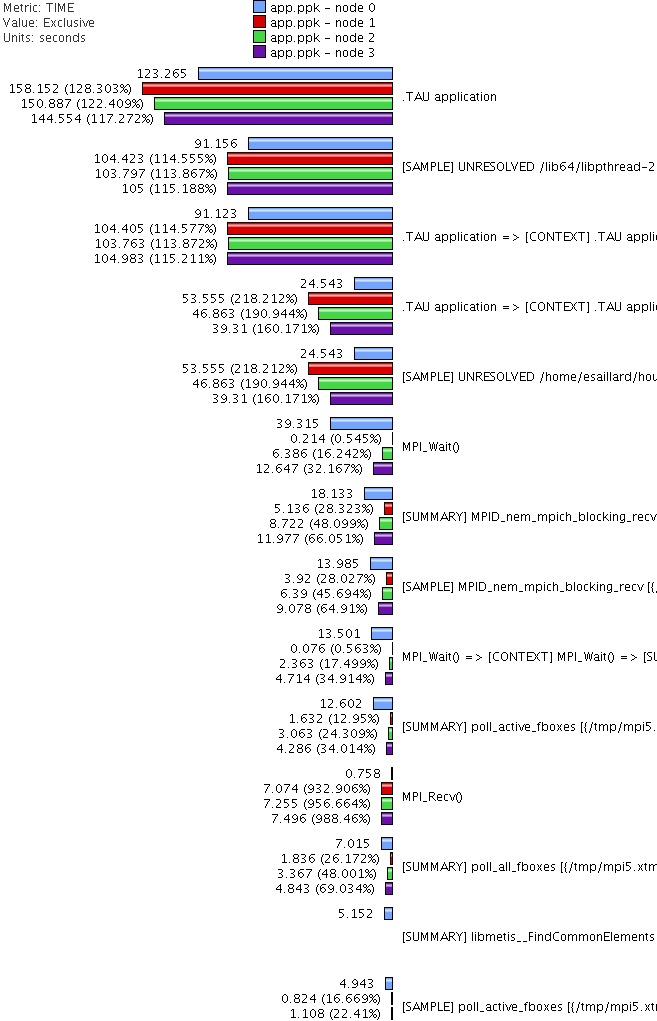
\includegraphics[width=14cm]{IMAGES/ScreenShot3}
\caption{Comparison window}
\label{fig:3}
\end{figure}


\noindent {\bf{3D Visualization}} \\

\begin{figure}[H]
\centering
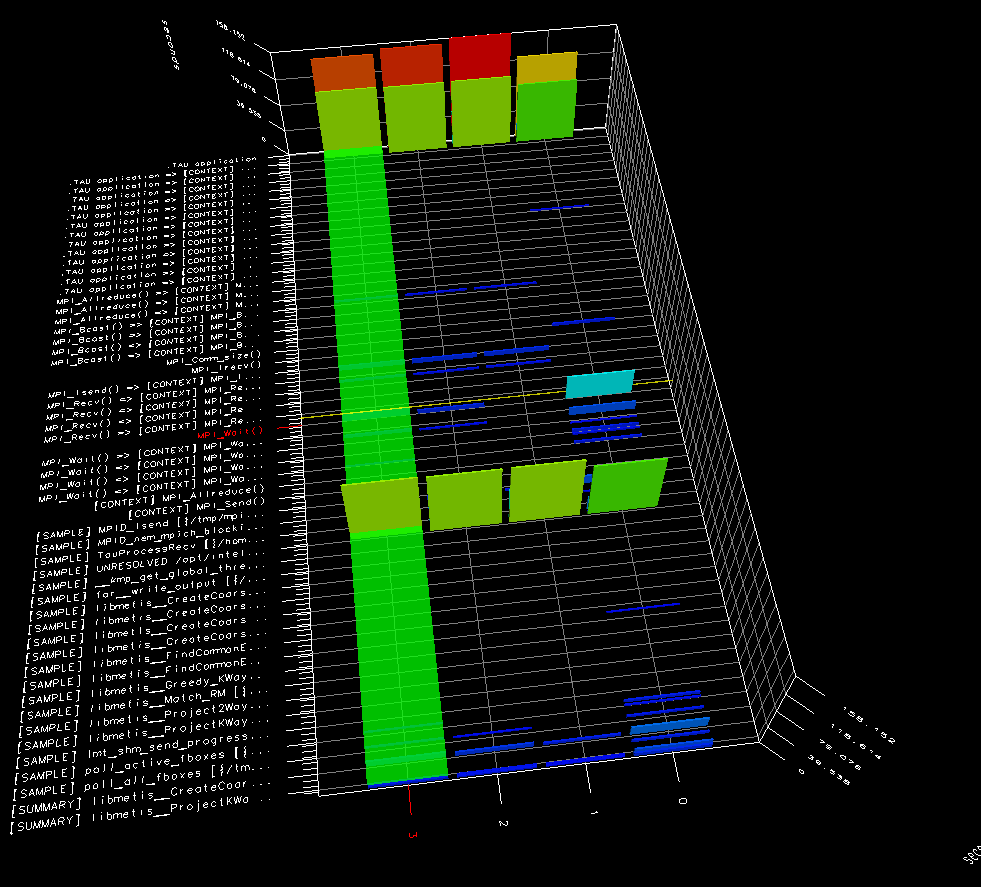
\includegraphics[width=10cm]{IMAGES/ScreenShot4}
\caption{3D Visualization}
\label{fig:4}
\end{figure}

A complete manual to use TAU and paraprof is available at \url{https://www.cs.uoregon.edu/research/tau/tau-usersguide.pdf}.


\section{Trace Analysis with Lucas and Arnaud's tool}

To use the tool, we first need to convert TAU traces to PAJE traces\footnote{For a tutorial on how to install tau2paje: https://github.com/schnorr/akypuera/wiki/TAUWithAkypuera}. After TAU generates tau.trc and tau.edf files, use tau2paje to generate tau.paje with the following command

\begin{cverbatim}
tau2paje --no-links --only-mpi --normalize-mpi tau.trc tau.edf > tau.paje
\end{cverbatim}

Then we use pj\_dump\footnote{For a tutorial on how to install pj dump: https://github.com/schnorr/pajeng/wiki/Install} to transform PAJE traces to CSV:

\begin{cverbatim}
pj_dump tau.paje | grep -e ^State -e ^Event > tau.csv
\end{cverbatim}

To check the head of the file: 

\begin{cverbatim}
head tau.csv
\end{cverbatim}

\subsection*{Analysis of the CSV using R+dplyr+ggplot2}

\lstset{language=R}
\begin{lstlisting}[caption=Code in R that analyses the CVS file (written in emacs using org mode)]
#+begin_src R :results output :session *R* :exports both  
library(dplyr);
df <- read.csv("tau.csv", header=FALSE, strip.white=TRUE);
# get only lines starting with State
df <- df %>% filter(V1 == "State");
names(df) <- c("Type", "Thread", "Type2", "Start", "End", "Duration", "Imbric", "Region");
df <- df %>% select(-Type, -Type2, -Duration, -Imbric);
df$Thread <- as.integer(gsub("rank", "", as.character(df$Thread)));
head(df);
#+end_src
\end{lstlisting}

\lstset{language=R}
\begin{lstlisting}[caption=Results]
#+RESULTS:
:   Thread    Start      End        Region
: 1      3 0.013019 0.037004      MPI_Init
: 2      3 0.038628 0.038630 MPI_Comm_size
: 3      3 0.038637 0.038637 MPI_Comm_rank
: 4      3 0.041826 0.046533     MPI_Bcast
: 5      3 0.046534 0.046543     MPI_Bcast
: 6      3 0.046546 0.046550     MPI_Bcast
\end{lstlisting}

\lstset{language=R}
\begin{lstlisting}[caption=Code in R that analyses the CVS file (written in emacs using org mode)]
#+begin_src R :results output :session *R* :exports both
library(ggplot2)
tstart = min(df$Start);
tend = max(df$End);

df %>%
  ggplot() + theme_bw(base_size=16) + xlab("Time [s]") +
  ylab("Thread") +
  theme(
     plot.margin = unit(c(0,0,0,0), "cm"),
     legend.margin = unit(.1, "line"),
     panel.grid = element_blank(),
     legend.position = "bottom",
     legend.title = element_blank()
   ) +
    coord_cartesian(xlim=c(tstart,tend)) +
    guides(fill = guide_legend(nrow = 2)) +
    geom_rect(alpha=1, aes(fill=Region,
                           xmin=Start,
                           xmax=End,
                           ymin=Thread,
                           ymax=Thread + 0.9))

tspan = tend - tstart;
tspan;
#+end_src
\end{lstlisting}

\lstset{language=R}
\begin{lstlisting}[caption=Results]
\end{lstlisting}
\vspace{-.5cm}

\begin{figure}[H]
\centering
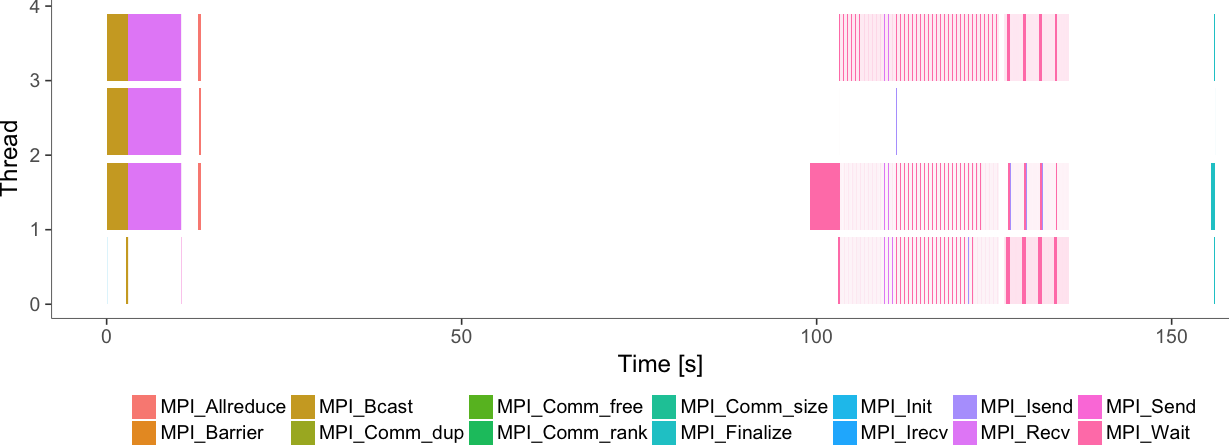
\includegraphics[width=13cm]{IMAGES/tool1}
\caption{Trace}
\label{fig:5}
\end{figure}

\lstset{language=R}
\begin{lstlisting}[caption=Code in R that analyses the CVS file (written in emacs using org mode)]
#+begin_src R :results output :exports both :session *R* 
df %>%
  filter(Start >= tstart, End <= tend) %>%
  group_by(Thread, Region) %>%
  summarize(count = length(End), TDur = sum(End-Start)/tspan*100) %>%
  group_by(Thread) %>%
  summarize(t=sum(TDur)) %>%
  as.data.frame();
#+end_src
\end{lstlisting}

\lstset{language=R}
\begin{lstlisting}[caption=Results]
#+RESULTS:
:   Thread         t
: 1      0  3.221339
: 2      1 11.986336
: 3      2  6.962705
: 4      3 10.838378
\end{lstlisting}


\section{Impact of input parameters}

The results presented in the previous section have been obtained with the following input parameters (file HPC4E.txt):

\begin{cverbatim}
3 Dimension
"MAILLAGES/florian3D" Nom du maillage
.H (.dat or .model)
0 p-adaptivity (no=0)
1 Ordre des elements
0 transient
0.01 Simulation Time
0.01 Time Step for the snapshots
0 HDG formulation (1=yes, 0=no)
10 Plane wave ...
1
1
40 30 50
430 30 50
680 1380 50
1
2
0 Do you want curved elements
1 Do you want to use mumps with symmetry
0 seismograms 
1 Type de CLA (1 pour du/dn=iomega u)
.false.
0 type RTM
0 Analytic Solution (0=no)
\end{cverbatim}


\subsection{Scalability}



To show the impact of input parameters, we can change the elements order in HPC4E.txt (\textit{Ordre des elements}) or refine the mesh (\texttt{tail MAILLAGES/florian3D.1.ele} will show the command). Beware of the total execution time, it takes into account the time spent to write in a file (time in function \texttt{sub\_time\_loop}).

\begin{table}[ht!]
\centering
\caption{Averaged of execution-Time (5 to 10 runs). {\underline{Input parameters}}: elements order =1, 859247 elements, {\bf{Simulation time=0.001}} (Time Step=0.001) - {\bf{without writting in sub\_time\_loop}}}
{\small
\begin{tabular}{|c|c|c|c|c|c|c|} \hline 
\multirow{2}{*}{ {{\bf{Number of MPI processes}}} }	& \multicolumn{3}{c|}{ {{\bf{Time spent in \texttt{sub\_time\_loop}  }}} }	& \multicolumn{3}{c|}{  {{\bf{Total execution time}}} }\\ 
										&  min 	& max	 & avg									& 	min & max & avg			\\ \hline \hline
 		4		                 				&  .7407	& .760 	& .746									&  	143.738 & 143.786	& 143.758 \\ \hline
 		8		                 				& .464	& .575  	& .512									&  	182.481 & 182.598 	& 182.554	\\ \hline		
 		16		                 				&  .142	& .174	 & .152									&  	215.348 & 215.398 	&  215.365\\ \hline
		 32		                 				& 1.288	&  5.884  & 4.011		  						        &  	293.542 &  293.639	& 293.619	\\ \hline
		64		                 				& 1.466	& 2.401 & 1.972									&  	360.580 & 360.936	& 360.886\\ \hline
\end{tabular}
}
\label{tab:1}
\end{table}


\begin{table}[ht!]
\centering
\caption{Averaged of execution-Time (5 to 10 runs). {\underline{Input parameters}}: elements order =1, 859247 elements,  {\bf{Simulation time=0.01}} (Time Step=0.01)  - {\bf{without writting in sub\_time\_loop}}}
{\small
\begin{tabular}{|c|c|c|c|c|c|c|} \hline 
\multirow{2}{*}{ {{\bf{Number of MPI processes}}} }	& \multicolumn{3}{c|}{ {{\bf{Time spent in \texttt{sub\_time\_loop}  }}} }	& \multicolumn{3}{c|}{  {{\bf{Total execution time}}} }\\ 
										&   		min & max & avg									& 	min & max & avg			\\ \hline \hline
 		4		                 				& 5.504 & 5.543 & 5.525										& 156.409 & 156.481 & 156.438 	\\ \hline
 		8		                 				& 2.652  &  2.686 &  2.665									&   175.770  &  175.813 &  175.786	\\ \hline
 		16		                 				&  1.612 & 1.660  & 1.631 									& 217.008 &  217.055 &  217.026	\\ \hline
		 32		                 				& .924 & .948   & .940										& 292.669  &  292.749 & 292.730	\\ \hline
		64		                 				& .430 & .444  & .438										&  356.742  & 357.0359 &  357.001	\\ \hline
\end{tabular}
}
\label{tab:2}
\end{table}


\begin{table}[ht!]
\centering
\caption{Averaged of execution-Time (5 to 10 runs). {\underline{Input parameters}}: elements order =1, 859247 elements,    {\bf{Simulation time=0.1}} (Time Step=0.1) - {\bf{without writting in sub\_time\_loop}}}
{\small
\begin{tabular}{|c|c|c|c|c|c|c|} \hline 
\multirow{2}{*}{ {{\bf{Number of MPI processes}}} }	& \multicolumn{3}{c|}{ {{\bf{Time spent in \texttt{sub\_time\_loop}  }}} }	& \multicolumn{3}{c|}{  {{\bf{Total execution time}}} }\\ 
										&   		min & max & avg									& 	min & max & avg			\\ \hline \hline
 		4		                 				& 55.325	& 55.344 & 55.333									&  194.500 & 194.522 & 194.512	\\ \hline
 		8		                 				& 26.804	& 26.843  & 26.820									&  200.059 & 200.105 & 200.083	\\ \hline
 		16		                 				&  17.671	&  17.710 & 17.688									&  233.131 & 233.162 &  233.145	\\ \hline
		 32		                 				& 9.779 & 9.803  & 9.794										&  301.450 & 301.533 & 301.514	\\ \hline
		64		                 				& 4.561 & 4.576  & 4.570										&  363.928 & 364.221 & 364.177	\\ \hline
\end{tabular}
}
\label{tab:3}
\end{table}



\subsection{Elements Order Variation}

Table \ref{tab:5} shows the total time and the time spent in function \texttt{sub\_loop\_time} for different elements orders, with 4 MPI processes. The times are obtained with the fortran function \texttt{CPU\_TIME}\footnote{Returns the CPU time, in seconds. If CPU\_TIME is used without any setting, the function returns the total user and system time for the current process.}. 
%The total execution time is obtained with \texttt{usr/bin/time}\footnote{Returns the elapsed real time between invocation and termination. The command is used with the -p option and the output format \%e (=elapsed real time in seconds).}.


\begin{table}[ht!]
\centering
\caption{Averaged of execution-Time (5 to 10 runs). {\underline{Input parameters}}: 859247 elements,  Simulation time=0.001 (Time Step=0.001) - {\bf{without writting in sub\_time\_loop}}}
{\small
\begin{tabular}{|c|c|c|c|c|c|c|} \hline 
\multirow{2}{*}{ {{\bf{Elements order}}} }	& \multicolumn{3}{c|}{ {{\bf{Time spent in \texttt{sub\_time\_loop}  }}} }	& \multicolumn{3}{c|}{  {{\bf{Total execution time}}} }\\ 
										&   		min & max & avg							& 	min & max & avg			\\ \hline \hline
 		1		                 				& 1.273 & 1.374 & 1.298								& 156.247  & 156.435 &  156.309	\\ \hline
 		2		                 				& 3.384	&  3.390  & 3.388							&  171.825 & 171.855 & 171.843		\\ \hline
 		3		                 				& 59.873 	 &  61.902	& 61.060							&  578.569 & 579.954 & 579.564 	\\ \hline
		 4		                 				& 39.003	& 39.288  & 39.156							& 527.505  & 527.555 & 527.528		\\ \hline
		5		                 				& 	&  &											&  	 & 	& 		\\ \hline
\end{tabular}
}
\label{tab:5}
\end{table}



\subsection{Mesh refinement}

To refine the mesh, we launch the following command

\begin{cverbatim}
./tetgen -kna10000A florian3D.poly
\end{cverbatim} 

\noindent and change the number in the option "-kna10000A".\\

Table \ref{tab:6} shows the total time and the time spent in function \texttt{sub\_loop\_time} for different mesh refinement, with 8 MPI processes.

\begin{table}[ht!]
\centering
\caption{Averaged of execution-Time (5 to 10 runs). {\underline{Input parameters}}: elements order=1, Simulation time=0.001 (Time Step=0.001)}
{\small
\begin{tabular}{|c|c|c|c|c|c|c|} \hline 
\multirow{2}{*}{ {{\bf{Mesh refinement}}} }	& \multicolumn{3}{c|}{ {{\bf{Time spent in \texttt{sub\_time\_loop}  }}} }	& \multicolumn{3}{c|}{  {{\bf{Total execution time}}} }\\ 
										&   		min & max & avg							& 	min & max & avg			\\ \hline \hline
 		10\ 000 (859\ 247 elt)		           	& .285 & .2973 &  .2917						&  175.0226 & 175.0522 & 175.041	\\ \hline
 		5\ 000 (1\ 704\ 052 elt)		                	& .8287 &  .8860 & .8590						&  348.888 & 379.0077 & 366.995	\\ \hline
 		2\ 500 (3\ 385\ 940 elt)	                		&  1.9168 &  1.9248	& 1.9214					&  708.008 & 707.994 &  707.993 \\ \hline
\end{tabular}
}
\label{tab:6}
\end{table}


%% Lancer avec 4 processus?? pour mieux comparer avec le reste


\section{Port hou10ni's kernel with BOAST}

This section presents how to install BOAST and use it to port Houdini's kernel. 

\subsection{How to install BOAST}

\begin{cverbatim}
git clone https://github.com/Nanosim-LIG/boast.git
cd boast
gem build BOAST.gemspec
gem install --user-install BOAST-2.0.3.gem 
\end{cverbatim}

\subsection{Original version}

The kernel is the loop over the fluid inner elements in \texttt{lib/libtransient/sub\_time\_loop.f90}. The loop is written outside of the code, in a new subroutine as presented below.

\lstset{language=FORTRAN}
\begin{lstlisting}[caption=kernel.f90]
SUBROUTINE fluid_inner_elt_ref(Nflu_inner, Nflusol_inner, nb_rhs, idx_vec_flu, idx_mat_flu, P_new, P_inter, P_old, A_flu, afluSize, pSize, vecSize_1, vecSize_2, matSize)
  implicit none
  INTEGER, PARAMETER :: dq=8 !< quadruple precision
  INTEGER, PARAMETER :: dp=4  !< double precision

  integer, intent(in) :: Nflu_inner
  integer, intent(in) :: Nflusol_inner
  integer, intent(in) :: nb_rhs
  integer, intent(in) :: afluSize
  integer, intent(in) :: pSize
  integer, intent(in) :: vecSize_1
  integer, intent(in) :: vecSize_2
  integer, intent(in) :: matSize
  INTEGER, INTENT(in), DIMENSION(vecSize_1,vecSize_2) :: idx_vec_flu
  INTEGER, INTENT(in), DIMENSION(matSize) :: idx_mat_flu
  REAL(kind=dp), INTENT(inout), DIMENSION(pSize,nb_rhs) :: P_new
  REAL(kind=dp), INTENT(in), DIMENSION(pSize,nb_rhs) :: P_inter
  REAL(kind=dp), INTENT(in), DIMENSION(pSize,nb_rhs) :: P_old
  REAL(kind=dp), INTENT(in), DIMENSION(afluSize) :: A_flu

  INTEGER :: I,J,I_tmp1,I_tmp2, I1, I2, I3, I4
  REAL(kind=dp), DIMENSION(20,nb_rhs) :: P_aux

  DO I=1,Nflu_inner+Nflusol_inner
    I_tmp1=1
    DO J=1,idx_vec_flu(1,I)
      I1=idx_vec_flu(2*J,I)
      I2=idx_vec_flu(2*J+1,I)
      I_tmp2=I_tmp1+I2-I1
      P_aux(I_tmp1:I_tmp2,1:nb_rhs)=P_inter(I1:I2,1:nb_rhs)
      I_tmp1=I_tmp2+1
    END DO
    I1=idx_vec_flu(2,I)
    I2=idx_vec_flu(3,I)
    I3=idx_mat_flu(I)
    I4=idx_mat_flu(I+1)-1

   P_new(I1:I2,1:nb_rhs)=MATMUL(RESHAPE(A_flu(I3:I4), (/I2-I1+1, I_tmp2/)),P_aux(1:I_tmp2,1:nb_rhs))-P_old(I1:I2,1:nb_rhs)
  END DO

END SUBROUTINE fluid_inner_elt_ref
\end{lstlisting}


\begin{lstlisting}[caption=sub\_time\_loop.f90]
SUBROUTINE sub_time_loop
...
CALL fluid_inner_elt(Nflu_inner, Nflusol_inner, nb_rhs, idx_vec_flu, idx_mat_flu, P_new, P_inter, P_old, A_flu, afluSize, pSize, vecSize_1, vecSize_2, matSize)
...
END SUBROUTINE 
\end{lstlisting}



To have an idea of the time spent in the kernel, table \ref{tab:7} shows the time of the entire function \texttt{sub\_time\_loop} (without the writing at the end) compared to the time spent in the kernel. Simulation time=0.01.

\begin{table}[H]
\centering
\caption{Time spent in the kernel (loop over fluid elements in {\tt sub\_time\_loop}), only one run - with an allocation at each step - {\bf{Avec l'ecriture des instantannees}}}
{\small
\begin{tabular}{|c|c|c|} \hline 
 {{\bf{Process ID}}} 	& {{\bf{Time in \texttt{sub\_time\_loop} }}}	& {{\bf{Time in \texttt{fluid\_inner\_elt} }}}\\ \hline \hline
		0		&   5.388336							&  5.1683220	(95,9\%)		\\ \hline 
 		1		&  5.352341							&  5.108320	(95,4\%)		\\ \hline
 		2		 &  5.360336							&  5.1203189	(95,5\%)		\\ \hline
		3		 &  5.412338 							&  5.1843260	(95,8\%)		\\ \hline	
\end{tabular}
}
\label{tab:7}
\end{table}

\begin{table}[H]
\centering
\caption{Time spent in the kernel (loop over fluid elements in {\tt sub\_time\_loop}), only one run - without allocation at each step - {\bf{Avec l'ecriture des instantannees}}}
{\small
\begin{tabular}{|c|c|c|} \hline 
 {{\bf{Process ID}}} 	& {{\bf{Time in \texttt{sub\_time\_loop} }}}	& {{\bf{Time in \texttt{fluid\_inner\_elt} }}}\\ \hline \hline
		0		&   4.776291							&  4.54828700	(95,2\%)		\\ \hline 
 		1		&  4.74029							&  4.5162959	(95,3\%)		\\ \hline
 		2		 &  4.744293							&  4.5242530	(95,4\%)		\\ \hline
		3		 & 4.768295 							&  4.53228600	(95\%)		\\ \hline	
\end{tabular}
}
\label{tab:8}
\end{table}


\subsection{Reference version}

We generate the exact same kernel as a reference version and run it with BOAST in order to compare the results in term of correctness and performances. KRef defines the reference version. This version simply needs to keep the Fortran code (referred as \texttt{codeF}) and wrap it with BOAST. To put it in a nutshell, a reference version should follow the template bellow.

\lstset{language=RUBY}
\begin{lstlisting}[caption=KRef\_template.rb]
def KRef
  lang = BOAST::get_lang
  BOAST::set_lang(BOAST::FORTRAN)
  kernel = BOAST::CKernel::new
  function_name = "function_ref"

  VARIABLES HERE
  FOR EXAMPLE : 
  geocode = BOAST::Int("geocode", :dir => :in )
  n01 = BOAST::Int("n01", :dir => :in)
  u = BOAST::Real("u", :dir => :in, :dim => [ BOAST::Dim(0, n01),  BOAST::Dim(0, n02))] )

   p = BOAST::Procedure::new(function_name, [geocode,n01,u])

   kernel.code.print <<EOF
  ORIGINAL C or FORTRAN CODE HERE
EOF

  kernel.procedure = p
  BOAST::set_lang(lang)
  return kernel
end

geocode = ...
n01 = ...
u = ...
k = KRef
stats = k.run(geocode, n01, u)
puts "#{k.procedure.name}: #{stats[:duration]*1.0e3}"
\end{lstlisting}



We wrote the reference version a bite differently as shown bellow.

\lstset{language=RUBY}
\begin{lstlisting}[caption=KRef.rb]
class KRef
 attr_reader :kernel

 def initialize(options)
  @opts = {:preprocessor => false, :unroll => false, :inline => :included}
  @opts.update(options)
  # Parameters 
  @Nflu_inner    = Int("Nflu_inner", :dir => :in )
  @Nflusol_inner = Int("Nflusol_inner", :dir => :in )
  @nb_rhs        = Int("nb_rhs", :dir => :in )
  @afluSize      = Int("afluSize", :dir => :in )
  @pSize         = Int("pSize", :dir => :in )
  @vecSize_1     = Int("vecSize_1", :dir => :in )
  @vecSize_2     = Int("vecSize_2", :dir => :in )
  @matSize       = Int("matSize", :dir => :in )
  @idx_vec_flu   = Int("idx_vec_flu", :dir => :in, :dim => [Dim(@vecSize_1),Dim(@vecSize_2)] )
  @idx_mat_flu   = Int("idx_mat_flu", :dir => :in, :dim => [Dim(@matSize)] )
  @P_new         = Real("P_new",:dir => :inout, :dim => [Dim(@pSize),Dim(@nb_rhs)])
  @P_inter       = Real("P_inter",:dir => :in, :dim => [Dim(@pSize),Dim(@nb_rhs)])
  @P_old         = Real("P_old",:dir => :in, :dim => [Dim(@pSize),Dim(@nb_rhs)])
  @A_flu         = Real("A_flu",:dir => :in, :dim => [Dim(@afluSize)])
 end

 def generate
  codeF = File::read("./kernel.f90")

  push_env(:lang => FORTRAN) {
     @kernel = CKernel:: new()
     @kernel.procedure = Procedure("fluid_inner_elt_ref",[@Nflu_inner, @Nflusol_inner, @nb_rhs, @idx_vec_flu, @idx_mat_flu, @P_new, @P_inter, @P_old, @A_flu, @afluSize, @pSize,@vecSize_1,@vecSize_2,@matSize] ,:functions => nil)
     get_output.print codeF
  }
   return @kernel
 end
 
end
\end{lstlisting}

The file run\_ref.rb is used to launch the kernel. 

\begin{lstlisting}[caption=run\_ref.rb]
require 'BOAST'
require './KRef.rb'
require 'narray_ffi'

include BOAST

 set_lang(FORTRAN)

# Creating ref kernel
k_ref_params = {:kernel => :ref, :LDFLAGS => "-lgfortran", :FCFLAGS => "-fbounds-check -O2"}
k = KRef::new(k_ref_params)
k.generate
puts k.kernel
k.kernel.build(:LDFLAGS => k_ref_params[:LDFLAGS], :FCFLAGS => k_ref_params[:FCFLAGS] )

# Parameters for loop iteration 1 and MPI Process 0 
# in the directory fluid_inner_elt_ref/sub_time_loop_1/
inputs = k.kernel.load_ref_inputs()
puts "** inputs =", inputs

inputs.each_key { |key|
  puts k.kernel.run(*(inputs[key]))
  puts k.kernel.compare_ref(outputs[key], inputs[key]).inspect
}

puts "Testing done\n"
\end{lstlisting}



\begin{lstlisting}[caption=Results (obtained with the command ruby run\_ref.rb)]
SUBROUTINE fluid_inner_elt_ref(Nflu_inner, Nflusol_inner, nb_rhs, idx_&
&vec_flu, idx_mat_flu, P_new, P_inter, P_old, A_flu, afluSize, pSize, v&
&ecSize_1, vecSize_2, matSize)
  implicit none
  INTEGER, PARAMETER :: dq=8 !< quadruple precision
  INTEGER, PARAMETER :: dp=4  !< double precision

  integer, intent(in) :: Nflu_inner
  integer, intent(in) :: Nflusol_inner
  integer, intent(in) :: nb_rhs
  integer, intent(in) :: afluSize
  integer, intent(in) :: pSize
  integer, intent(in) :: vecSize_1
  integer, intent(in) :: vecSize_2
  integer, intent(in) :: matSize
  INTEGER, INTENT(in), DIMENSION(vecSize_1,vecSize_2) :: idx_vec_flu
  INTEGER, INTENT(in), DIMENSION(matSize) :: idx_mat_flu
  REAL(kind=dp), INTENT(inout), DIMENSION(pSize,nb_rhs) :: P_new
  REAL(kind=dp), INTENT(in), DIMENSION(pSize,nb_rhs) :: P_inter
  REAL(kind=dp), INTENT(in), DIMENSION(pSize,nb_rhs) :: P_old
  REAL(kind=dp), INTENT(in), DIMENSION(afluSize) :: A_flu

  !! Variables declaration
  INTEGER :: I,J,I_tmp1,I_tmp2, I1, I2, I3, I4
  REAL(kind=dp), DIMENSION(20,nb_rhs) :: P_aux

  DO I=1,Nflu_inner+Nflusol_inner
    I_tmp1=1
    DO J=1,idx_vec_flu(1,I)
      I1=idx_vec_flu(2*J,I)
      I2=idx_vec_flu(2*J+1,I)
      I_tmp2=I_tmp1+I2-I1
      P_aux(I_tmp1:I_tmp2,1:nb_rhs)=P_inter(I1:I2,1:nb_rhs)
      I_tmp1=I_tmp2+1
    END DO
    I1=idx_vec_flu(2,I)
    I2=idx_vec_flu(3,I)
    I3=idx_mat_flu(I)
    I4=idx_mat_flu(I+1)-1

   P_new(I1:I2,1:nb_rhs)=MATMUL(RESHAPE(A_flu(I3:I4), (/I2-I1+1, I_tmp&
&2/)),P_aux(1:I_tmp2,1:nb_rhs))-P_old(I1:I2,1:nb_rhs)
  END DO

END SUBROUTINE fluid_inner_elt_ref

** inputs =
{"./fluid_inner_elt_ref/sub_time_loop_1"=>[210025, 0, 1, NArray.int(2577732): 
[ 5, 1, 4, 538597, 538600, 319233, 319236, 363785, 363788, 665493, ... ], NArray.int(214812): 
[ 1, 81, 161, 209, 289, 369, 449, 529, 609, 689, 769, 849, 913, 993, ... ], NArray.float(439866): 
[ 0.0, 0.0, 0.0, 0.0, 0.0, 0.0, 0.0, 0.0, 0.0, 0.0, 0.0, 0.0, 0.0, 0.0, ... ], NArray.float(439866): 
[ 0.0, 0.0, 0.0, 0.0, 0.0, 0.0, 0.0, 0.0, 0.0, 0.0, 0.0, 0.0, 0.0, 0.0, ... ], NArray.float(439866): 
[ 0.0, 0.0, 0.0, 0.0, 0.0, 0.0, 0.0, 0.0, 0.0, 0.0, 0.0, 0.0, 0.0, 0.0, ... ], NArray.float(8476280): 
[ 1.1026e-18, 9.61982e-17, 1.0165, 9.2055e-17, 9.13418e-19, 9.01442e-17, ... ], 16952560, 879732, 12, 214811, 214812]}

{:duration=>0.153594073}
\end{lstlisting}



\subsection{BOAST version}

\lstset{language=RUBY}
\begin{lstlisting}[caption=KBoast.rb]
class KBoast
 attr_reader :kernel

 def initialize(options)

  # Parameters 
  @Nflu_inner         = Int("Nflu_inner", :dir => :in )
  @Nflusol_inner      = Int("Nflusol_inner", :dir => :in )
  @nb_rhs             = Int("nb_rhs", :dir => :in )
  @afluSize           = Int("afluSize", :dir => :in )
  @pSize              = Int("pSize", :dir => :in )
  @vecSize_1          = Int("vecSize_1", :dir => :in )
  @vecSize_2          = Int("vecSize_2", :dir => :in )
  @matSize            = Int("matSize", :dir => :in )
  @idx_vec_flu        = Int("idx_vec_flu", :dir => :in, :dim => [Dim(@vecSize_1),Dim(@vecSize_2)] )
  @idx_mat_flu        = Int("idx_mat_flu", :dir => :in, :dim => [Dim(@matSize)] )
  @P_new              = Real("P_new",:dir => :inout, :dim => [Dim(@pSize),Dim(@nb_rhs)])
  @P_inter            = Real("P_inter",:dir => :in, :dim => [Dim(@pSize),Dim(@nb_rhs)])
  @P_old              = Real("P_old",:dir => :in, :dim => [Dim(@pSize),Dim(@nb_rhs)])
  @A_flu              = Real("A_flu",:dir => :in, :dim => [Dim(@afluSize)])

 end

 def generate

   push_env(:lang => FORTRAN) {

    @kernel = CKernel:: new()
    @kernel.procedure = Procedure("fluid_inner_elt_boast",[@Nflu_inner, @Nflusol_inner, @nb_rhs, @idx_vec_flu, @idx_mat_flu, @P_new, @P_inter, @P_old, @A_flu, @afluSize, @pSize,@vecSize_1,@vecSize_2,@matSize] ,:functions => nil)

    #..  FUNCTIONS ..#
    register_funccall("matmul") if get_lang == FORTRAN
    call_matmul = lambda{|x,y|
        return matmul(x,y)
    }

    #.. KERNEL ..#

    opn @kernel.procedure

    # local variables
    i = Variable::new('I', Int)
    j = Variable::new('J', Int)
    i_tmp1 = Variable::new('I_tmp1', Int)
    i_tmp2 = Variable::new('I_tmp2', Int)
    i1 = Variable::new('I1', Int)
    i2 = Variable::new('I2', Int)
    i3 = Variable::new('I3', Int)
    i4 = Variable::new('I4', Int)
    p_aux = Variable::new("P_aux",Real, :dimension => [Dim(20),Dim(@nb_rhs)])

    decl i,j,i_tmp1,i_tmp2, i1,i2,i3,i4,p_aux

    pr For(i,1,@Nflu_inner+@Nflusol_inner){
      pr i_tmp1 === 1
      pr For(j,1,@idx_vec_flu[1,i]){
        pr i1 === @idx_vec_flu[2*j,i]
        pr i2 === @idx_vec_flu[2*j+1,i]
        pr i_tmp2 === i_tmp1 + i2 - i1
        pr p_aux.slice(i_tmp1..i_tmp2,1..@nb_rhs) === @P_inter.slice(i1..i2,1..@nb_rhs) 
        pr i_tmp1 === i_tmp2 +1
      }
      pr i1 === @idx_vec_flu[2,i]
      pr i2 === @idx_vec_flu[3,i]
      pr i3 === @idx_mat_flu[i]
      pr i4 === @idx_mat_flu[i+1] - 1
      reshape_code ="RESHAPE(#{@A_flu.slice(i3..i4)}, (/#{i2}-#{i1}+1, #{i_tmp2}/))"
      pr @P_new.slice(i1..i2,1..@nb_rhs) === call_matmul.call(reshape_code , p_aux.slice(1..i_tmp2,1..@nb_rhs) ) - @P_old.slice(i1..i2,1..@nb_rhs)
    }
    close @kernel.procedure
   }

   return @kernel
 end
end
\end{lstlisting}


\noindent The file run\_boast.rb is used to launch the BOAST version of the kernel. We run 3 times the kernel (repeat). \\

\begin{lstlisting}[caption=run\_boast.rb]
require 'BOAST'
require './KBoast.rb'
require 'narray_ffi'

include BOAST

set_default_real_size(4)

k_boast_params = {:kernel => :boast, :LDFLAGS => "-lgfortran", :FCFLAGS => "-fbounds-check -fimplicit-none -O2"}  

set_lang(FORTRAN)
stats = []
repeat = 5

# Creating boast kernel
k = KBoast::new(k_boast_params)
k.generate
puts k.kernel
k.kernel.build(:LDFLAGS => k_boast_params[:LDFLAGS], :FCFLAGS => k_boast_params[:FCFLAGS] )
 
inputs = k.kernel.load_ref_inputs()
outputs = k.kernel.load_ref_outputs()

inputs.each_key { |key|
  repeat.times {
    stats.push k.kernel.run(*(inputs[key]))
  }
  puts k.kernel.compare_ref(outputs[key], inputs[key]).inspect
}

stats.sort_by! { |a| a[:duration] }
p stats
stats = stats.first

puts "#{k.kernel.procedure.name}: optim_nested = #{k_boast_params[:optim_nested]}  #{stats[:duration]} s ->  #{stats[:duration]*1.0e3} ms"
\end{lstlisting}


\begin{lstlisting}[caption=Results (obtained with the command ruby run\_boast.rb)]
SUBROUTINE fluid_inner_elt_boast(Nflu_inner, Nflusol_inner, nb_rhs, idx_&
&vec_flu, idx_mat_flu, P_new, P_inter, P_old, A_flu, afluSize, pSize, v&
&ecSize_1, vecSize_2, matSize)

  integer, parameter :: wp=kind(1.0d0)
  integer(kind=4), intent(in) :: Nflu_inner
  integer(kind=4), intent(in) :: Nflusol_inner
  integer(kind=4), intent(in) :: nb_rhs
  ...
  
END SUBROUTINE fluid_inner_elt_boast

{"P_new"=>0.0}
[{:duration=>0.011553553000000001, :start=>-8096482666880853504, :end=>-8084929113880853504}, {:duration=>0.011923121, :start=>-8122491033880853504, :end=>-8110567912880853504}, {:duration=>0.013262399000000001, :start=>-8135791916880853504, :end=>-8122529517880853504}, {:duration=>0.013991319, :start=>-8110525936880853504, :end=>-8096534617880853504}, {:duration=>0.014984313, :start=>-8150824959880853504, :end=>-8135840646880853504}]
fluid_inner_elt_boast: optim_nested = 3  0.011553553000000001 s ->  11.553553 ms
\end{lstlisting}


\subsection{Optimisations}


Unroll both loops.



\lstset{language=RUBY}
\begin{lstlisting}[caption=KBoast.rb]
class KBoast
 attr_reader :kernel


 def initialize(options)

  @opts = {:optim_nested => 1, :optim_main => 1}
  @opts.update(options)

  # Parameters 
  @Nflu_inner         = Int("Nflu_inner", :dir => :in )
  @Nflusol_inner      = Int("Nflusol_inner", :dir => :in )
  @nb_rhs             = Int("nb_rhs", :dir => :in )
  @afluSize           = Int("afluSize", :dir => :in )
  @pSize              = Int("pSize", :dir => :in )
  @vecSize_1          = Int("vecSize_1", :dir => :in )
  @vecSize_2          = Int("vecSize_2", :dir => :in )
  @matSize            = Int("matSize", :dir => :in )
  @idx_vec_flu        = Int("idx_vec_flu", :dir => :in, :dim => [Dim(@vecSize_1),Dim(@vecSize_2)] )
  @idx_mat_flu        = Int("idx_mat_flu", :dir => :in, :dim => [Dim(@matSize)] )
  @P_new              = Real("P_new",:dir => :inout, :dim => [Dim(@pSize),Dim(@nb_rhs)])
  @P_inter            = Real("P_inter",:dir => :in, :dim => [Dim(@pSize),Dim(@nb_rhs)])
  @P_old              = Real("P_old",:dir => :in, :dim => [Dim(@pSize),Dim(@nb_rhs)])
  @A_flu              = Real("A_flu",:dir => :in, :dim => [Dim(@afluSize)])

 end
 
  def generate

   push_env(:lang => FORTRAN) {

   @kernel = CKernel:: new()
   @kernel.procedure = Procedure("fluid_inner_elt_boast",[@Nflu_inner, @Nflusol_inner, @nb_rhs, @idx_vec_flu, @idx_mat_flu, @P_new, @P_inter, @P_old, @A_flu, @afluSize, @pSize,@vecSize_1,@vecSize_2,@matSize] ,:functions => nil)


    #..  FUNCTIONS ..#

    register_funccall("matmul") if get_lang == FORTRAN
    call_matmul = lambda{|x,y|
        return matmul(x,y)
    }

    register_funccall(:modulo) if get_lang == FORTRAN


    #.. KERNEL ..#

    opn @kernel.procedure

    # local variables
    i = Variable::new('I', Int)
    j = Variable::new('J', Int)
    i_tmp1 = Variable::new('I_tmp1', Int)
    i_tmp2 = Variable::new('I_tmp2', Int)
    i1 = Variable::new('I1', Int)
    i2 = Variable::new('I2', Int)
    i3 = Variable::new('I3', Int)
    i4 = Variable::new('I4', Int)
    p_aux = Variable::new("P_aux",Real, :dimension => [Dim(20),Dim(@nb_rhs)])

    jmax = Variable::new('jmax', Int)
    imax = Variable::new('imax', Int)

    decl i,j,i_tmp1,i_tmp2, i1,i2,i3,i4,p_aux
    decl jmax,imax


    ##.. Nested loop optimization
    optim_1 = lambda { |unroll,i|
      loop_1 = lambda { |indice|
        pr i1 === @idx_vec_flu[2*indice,i]
        pr i2 === @idx_vec_flu[2*indice+1,i]
        pr i_tmp2 === i_tmp1 + i2 - i1
        pr p_aux.slice(i_tmp1..i_tmp2,1..@nb_rhs) === @P_inter.slice(i1..i2,1..@nb_rhs)
        pr i_tmp1 === i_tmp2 + 1.to_var
      }

      pr jmax === @idx_vec_flu[1,i]-(unroll-1)
      f_nested = For(j,1,jmax, step: unroll){
        unroll.times { |k|
          loop_1[j+k]
        }
      }
      f_arr_nested = [f_nested]
      if unroll > 1 then
          f2_nested = For(j,(@idx_vec_flu[1,i]-modulo(@idx_vec_flu[1,i],unroll))+1, @idx_vec_flu[1,i]){
            loop_1[j]
          }
          f_arr_nested.push f2_nested
      end
      f_arr_nested
   }


    ##.. Main loop optimization
    optim_2 = lambda { |unroll|
      loop_2 = lambda { |indice|
        pr i_tmp1 === 1
        # Nested loop optimized - No optimization -> = optim_1[1,indice].each{ |f|  pr f }
        optim_1[@opts[:optim_nested],indice].each { |f_nested|
          pr f_nested
        }
        pr i1 === @idx_vec_flu[2,indice]
        pr i2 === @idx_vec_flu[3,indice]
        pr i3 === @idx_mat_flu[indice]
        pr i4 === @idx_mat_flu[indice+1] - 1
        reshape_code ="RESHAPE(#{@A_flu.slice(i3..i4)}, (/#{i2}-#{i1}+1, #{i_tmp2}/))"
        pr @P_new.slice(i1..i2,1..@nb_rhs) === call_matmul.call(reshape_code , p_aux.slice(1..i_tmp2,1..@nb_rhs) ) - @P_old.slice(i1..i2,1..@nb_rhs)
      }

      pr imax === @Nflu_inner+@Nflusol_inner-(unroll-1)
      f_main = For(i,1,imax, step: unroll){
        unroll.times { |k|
          loop_2[i+k]
        }
      }
      f_arr_main = [f_main]
      if unroll > 1 then
        f2_main = For(i,(@Nflu_inner+@Nflusol_inner-modulo(@Nflu_inner+@Nflusol_inner,unroll))+1, @Nflu_inner+@Nflusol_inner){
          loop_2[i]
        }
        f_arr_main.push f2_main
      end
      f_arr_main
    }



    ## Procedure
    optim_2[@opts[:optim_main]].each { |f_main|
        pr f_main
    }

    close @kernel.procedure
   }

   return @kernel
 end    
end 
\end{lstlisting}






\section{Comparison between MPI and MPI+OpenMP versions of hou10ni}
TODO

\end{document}
